\begin{figure}[t!]
 \begin{center}
   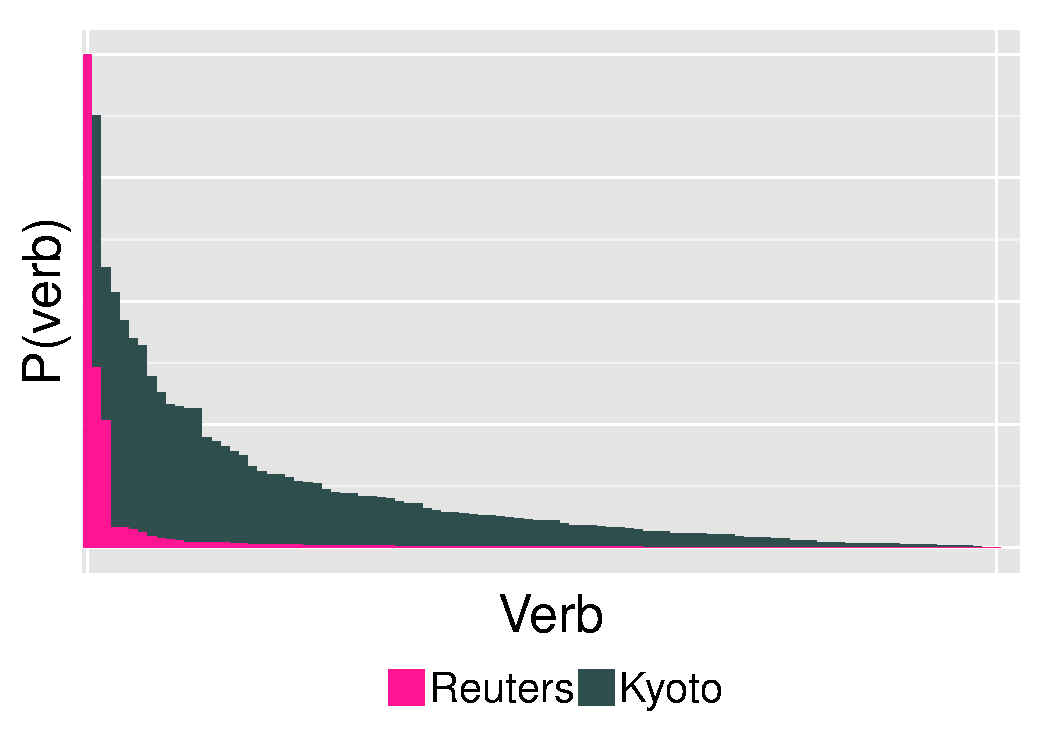
\includegraphics[width=1.0\linewidth]{2016_conll_verbpred/figures/top100verbs_kyoto_hist_no_suru-iru-aru-naru}
   \caption{Distribution of the top 100 content verbs in the Kyoto corpus and
     the Reuters Japanese news corpus.  Both are Zipfian, but the Reuters corpus
     is even more skewed, even with the common special cases
     excluded.}
 \label{fig:hist}
  \end{center}
\end{figure}

Now that we have the results of the previous section, we have
baselines against which we can compare computational verb prediction
approaches.  In this section, we introduce incremental verb
classification with a linear classifier.\footnote{While we use
  logistic regression, using hinge loss achieves similar accuracy.}
For our investigation of computational verb classification, we use two
very different languages that both have verb-final syntax---Japanese,
which is agglutinative, and German, which is not---and show that
discriminative classifiers can predict final verbs with increasing
accuracy as more context of sentences is revealed.

A simple verb prediction scheme applied to German~\cite{grissom2014}
achieves poor accuracy.  Their approach creates a Kneser-Ney \ngram{}
language model for the prior context associated with each verb in the
corpus; i.e., 50 $n$-gram models for 50 verbs. Given pre-verb $n$-gram
context $c$ in a sentence $S_t$, and verb prediction $v^{(t)}\in V$,
the verb selection is defined by the following equation:
\begin{equation}
  \label{eq:ngram}
  v^{(t)} \equiv \arg \max_v \prod_{c \in S_t} p(c \g v) p(v).
\end{equation}

It chooses the verb that maximizes the probability of the observed
context, scaled by the prior probability of the verb in the overall
corpus. Unsurprisingly, given the distribution of verbs in real data
(Figure~\ref{fig:hist}), this \ngram{}-based approach has low accuracy
and tends to predict the most common verb. For a translation system,
this often degenerates into the less interesting problem of whether to
trust whether the final verb is indeed a common one.  While this
improves translation delay, better predictions will lead to more
significant improvements.  We instead opt for a one-vs-all
discriminative classification approach.\footnote{One-vs-all
  classification builds a classifier for each class versus the
  aggregate all other classes.} 
\begin{figure}[t!]
  \begin{center} 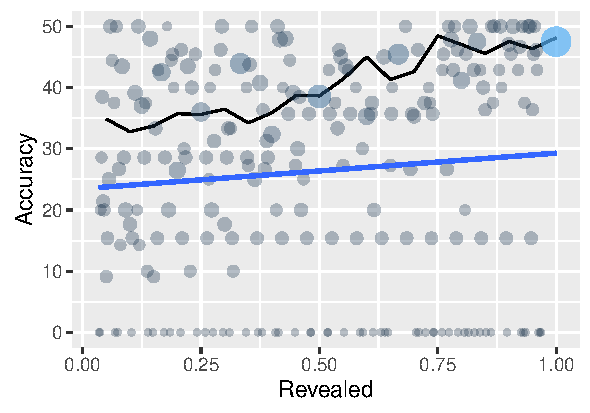
\includegraphics[width=1.0\linewidth]{2016_conll_verbpred/figures/CF_classify} \caption{Verb
      classification results on crowdsourced sentences. Despite many
      out-of-vocabulary items and significant noise, the average
      accuracy, shown in the non-monotonic line in the plot, increases
      over the course of the sentence. Larger, darker circles indicate
      more examples for a given position.  Accuracy was calculated by
      aggregating the guesses at 5\% intervals. }
\label{fig:CF_classify}
\end{center}
\end{figure}

\subsection{Classification on Human Data}
\label{sec:cf_classify}

We first incrementally classify verbs on the same 200 sentences from
Section~\ref{sec:human}.  Since the answer choices are often complex
verb \textit{bunsetsu} and since many of these verb phrase answer
choices do not appear among the most common verbs, lemmatizing the
verbs and performing one-vs-all classification yields extremely low
accuracy. Thus, we use binary classification with a single linear
classifier to produce a probability for each candidate answer,
encoding the verb phrase itself into the feature vector.

\subsubsection{Training a Morphological Model}
The processing is as follows: We train on 463,716 verb-final sentences
extracted from the training data.  We use both \textbf{context
  features} and \textbf{final verb features}.  Our context features,
i.e., those preceding the final verb, are represented as follows: the
context \textbf{unigrams} and \textbf{bigrams} take a value of $1$ if
they are present and $0$ otherwise; \textbf{case markers} observed in
the sentence context are represented as unigrams and bigrams in the
order that they appear; and we reserve a distinct feature for the
\textbf{last observed case marker} in the sentence.  Our \textbf{verb
  features} consist of the final verb's tokens given by the
morphological analyzer, which, in addition to the verb stem itself,
typically include tense and aspect information.  These are represented
as unigrams and bigrams in the feature vector.

To allow the classifier to learn, we must encode the interactions
between the verb features and the context features.  Thus, we
use the Cartesian product of sentence and verb features to encode
interactions between them: for each training sentence we generate
both a positive and a negative example. The example with the correct
verb phrase is labeled as a positive example ($+1$), and we uniformly
select a random verb phrase from one of the 500 most common verb
phrases and label it as negative ($-1$) example for the same sentence
context,\footnote{We experimented with several numbers of weighted
  negative examples and found that one negative example with of equal
  weight to the positive gave the best results of the configurations
  we tried.}  yielding 927,432 training examples and 267,037,571
features.


For clarity, we describe this feature representation more
formally. Given sentence $S_t$ with a pre-verb context consisting of
unigrams, bigrams, and case marker tokens, $C=\{c_0, ..., c_n\}$, and
\textit{bunsetsu} verb phrase tokens $A=\{a_0, ..., a_k\}$, the
feature vector consists of
$C\times A = \{c_0\wedge a_0, c_0\wedge a_1, ..., c_n\wedge a_k\}$,
where $\wedge$ concatenates the two context and answer strings.
During learning, the weights learned for the concatenated tokens are
thus based on the relationship between a context token and a
\textit{bunsetsu} token and mapped to $\{+1,-1\}$.  More concretely,
individual morphemes of the Japanese verb phrase are combined with the
pre-verb unigrams, bigrams, and uniquely identified case marker
tokens.  Accuracy improves when the morphemes used in the negative
examples and positive examples are disjoint; so, we enforce this
constraint when selecting negative examples. For example, if the
positive example includes the past tense morpheme, た, the negative
example is altogether disallowed from having this morpheme as a verb
feature.  
\subsubsection{Choosing an Answer}
At test time, we test progressively longer fragments of each sentence,
extracting the aforementioned features online until the entire
pre-verb context is available. For every sentence fragment, the
classifier determines the probability of each of the four possible
verbs by adding their verb features to the feature vector of the
example.  The answer choice with the highest probability of $+1$ (or
the lowest probability of $-1$) is chosen as the answer. By taking
this approach, we can model complex verbs and their context jointly.
Intuitively, the probability of a ($+1$) is the model's prediction of
how well the \textit{bunsetsu} verb phrase fits with the sentence
context (represented by the feature vector).

Some verbs are absent from the training data, forcing the classifier
to rely on morphemes to distinguish between them.  The
alternative---e.g., in a typical one-vs-all classification
approach---is that the classifier could reason from nothing whatsoever
when a fully-inflected verb is absent from the training data. Given
the complexity of \textit{bunsetsu}, this happens often even in large
corpora for a language such as Japanese.






\subsubsection{Multiple Choice Results}
Despite only choosing among four choices, this task is in many ways
more difficult than the 50-label classification problem described in
the next section because of the added complexity inherent modeling the
effect of morphemes and missing examples.  These limitations
notwithstanding, the accuracy does improve as more of the sentence is
revealed (Figure~\ref{fig:CF_classify}), indicating that the algorithm
learns to use these features to rank verbs, though the performance
significantly lags that of both the human participants and our later
experiments. 





Additionally, on the \textbf{full context set}, sentence length is
negatively correlated with accuracy
(Figure~\ref{fig:CF_classifier_length}), as in the much more
convincing results of our human experiments
(Figure~\ref{fig:full_prefix}), though the trend is not entirely
consistent, making it difficult to draw firm conclusions.  Case
density is again positively correlated with accuracy on both the
random (Figure~\ref{fig:CF_case_density}) and full context sets.
\begin{figure}[t!]
  \begin{center} 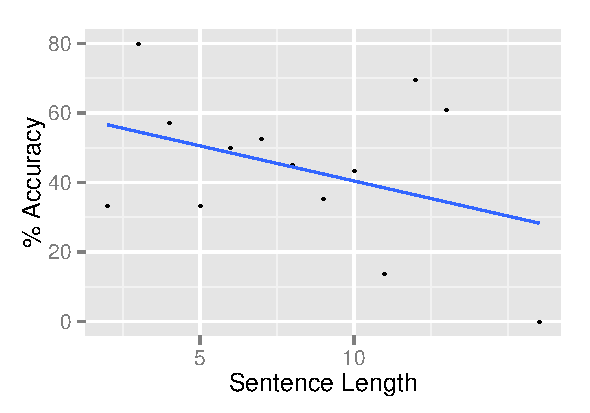
\includegraphics[width=1.0\linewidth]{2016_conll_verbpred/figures/CF_len_run2} \caption{
      Classification accuracy as a function of sentence length on the
      full context set. While there is a clear correlation between
      sentence length and accuracy, there are several
      outliers. Compare to Figure~\ref{fig:full_prefix}.}
\label{fig:CF_classifier_length}
\end{center}
\end{figure}

\paragraph{An Illustrative Example}

To gain some insight into how features can influence the classifier,
we here examine an example of the classifier's behavior on the
multiple choice data.

\begin{enumerate}[(5)]
\listsep
\item \label{sent-class}
\gl{少年時代-は}{childhood days-\abr{top}}
\gl{\hspace{2.5em}熊本藩-の}{Kumamoto domain-\abr{gen}}
\gl{藩校-で}{clan school-\abr{loc}}
\gl{儒学-を}{Confucianism-\abr{acc}}
\gl{学び、}{study:\abr{med}}
\gl{後-に}{subsequently-\abr{loc}}
\gl{西本願寺-において}{Nishihongan Temple-\abr{loc}}
\gl{修行-に}{discipline-\abr{all}}
\end{enumerate}
\begin{enumerate}[(6)]
\listsep
\item \label{sent-class-choices}
\begin{enumerate*}
  \item \gl{励ん-だ}{strive-PAST}
  \item \gl{創刊-さ-れ-る}{issue-do-PASS-NPST}
  \item \gl{加え-られ-てい-る}{add-PASS-CONT-NPST}
  \item \gl{勤め-る}{serve-NPST}
\end{enumerate*}
\end{enumerate}
In Example (5), the classifier incorrectly chooses ``issue'' as the
verb until observing the accusative case marker attached to
``Confucianism''.  At this point, the classifier's confidence in the
correct answer rises to 0.74---and correctly chooses ``strive''.  This
answer goes unchanged for the remainder of the sentence, though
``study'' attaches to ``Confucianism'', not the final verb. The
combined evidence, however, is enough for the classifier to select
correctly, and indeed, most of the following tokens only increase the
classifier's confidence.  Adding ``subsequently'' increases confidence
to 0.84, an intuitive increase given the likely tense information
contained in such a word.  The somewhat redundant case marker here
only increases confidence to 0.86.  Adding the reference to the temple
decreases confidence again to 0.79.  But adding the \textbf{final case
  marker}, which also forms a new bigram with the previous word,
results in a huge increase in confidence, to 0.90.

\subsection{Multiclass Verb Prediction}

\begin{figure}[t!]
  \begin{center} 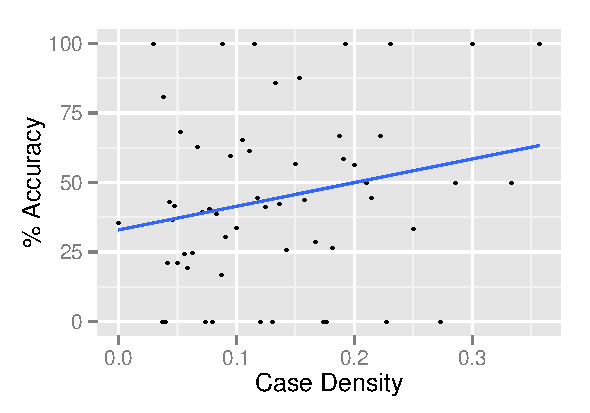
\includegraphics[width=1.0\linewidth]{2016_conll_verbpred/figures/CF_density_incremental} \caption{
      Classification accuracy as a function of case density on the
      incremental sentences.  The accuracy is correlated with case density,
      but the data are extremely noisy.  Full-context accuracy has a
      similar trend (not shown).}
\label{fig:CF_case_density}
\end{center}
\end{figure}

While the multiple choice experiment was more open-ended (predicting
random verbs), we now focus on a more constrained task: how well can
we predict the most frequent verbs.  This is the central conceit of
\newcite{grissom2014}: if you can do a good job of this, you can
improve simultaneous translation.  They show a slight improvement in
simultaneous translation by using \ngram{} language model-based verb
prediction.  We show a large improvement over their approach to verb
prediction using a discriminative multiclass logistic
classifier~\cite{langford2007vowpal}.

\paragraph{Data Preparation}

Our classes for multiclass classification are the fifty most common
verbs in the \abr{kft} (Japanese, as in the human study) and
Wortschatz corpora~\cite[German]{biemann2007leipzig}.

We use data from the training and test sets of the \abr{kft} Japanese
corpus of Wikipedia articles and a random split of the German
Wortschatz web corpus, from which we extract the verb-final
sentences. \newcite{grissom2014} use an \ngram{} model to distinguish
between the fifty most common German verbs for \abr{sov}-\abr{svo}
simultaneous machine translation, which we replicate as our baseline.
Following this study, we train a model on the fifty most common verbs
in the training set.

In Japanese, due to the small size of the standard test set, we
split the data randomly, training on 60,926 verb-final
sentences ending in the top fifty verbs and testing on 1,932.  Our total
feature count is 4,649,055.  We use the MeCab~\cite{kudo2005mecab}
morphological analyzer for segmentation and verb identification.  We
consider only verb-final sentences. We skip semantically vacuous
post-verbal copulas when identifying final verbs.

\paragraph{Finding Verbs}

We identify verbs in the German text with a part-of-speech
tagger~\cite{toutanova2003feature} and select from the top fifty
verbs.  We consider the sentence-ending set of verbs to be the final
verbs. We train on 76,209 verb-final sentences ending in the top fifty
verbs and test on 9,386.  In German, to approximate the case
information that we extract in Japanese, we test the inclusion of
equivalent unigram and bigram features for German \textbf{articles},
the surface forms of which determine the case of the next noun phrase.

In Japanese, we omit some special cases of light verbs that combine
with other verbs, as well as ambiguous surface forms and
copulas.\footnote{In Japanese, we omit some ambiguous cases and
  variants of ``is'' and ``do'': excluded are variants of
  \textit{suru} (``to do''), which combines with nouns to form new
  verbs, \textit{aru} (``is'', inanimate case), and \textit{iru}
  (``is'', animate case). The tokens \textit{aru} and \textit{iru}
  also combine with other verbs to change tense and aspect, in which
  case they are not verbs, and can form the copula \textit{de aru}.
  Distinguishing between all of these cases is beyond the scope of
  this study; so, they are excluded.  We also omit duplicates that are
  spelled differently (i.e., the same word but spelled without Chinese
  (\textit{kanji}) characters and slightly different forms of the same
  root).

  We also omit the light verb \textit{naru} (``to become'' or ``to
  make up'') for similar reasons to \textit{suru}.  The increasing
  trend shown in the results does not change with their inclusion.}

\paragraph{Features}

All features are encoded as binary features indicating their presence
or absence.  For Japanese, we again include \textbf{case unigrams},
and \textbf{case bigrams}, which encode as distinct features the for
case markers observed thus far.\footnote{For instance, given a
  sentence fragment X-に Y-を, representing X-\abr{dat} Y-\abr{acc},
  the case bigram would be に$\wedge$を.}  We also include a feature
for the \textbf{last observed case marker}.  For both Japanese and
German, we normalize the verbs to the non-past, plain form, both
providing more training data for each verb and simplifying the job of
our classifier.

German case is conveyed primarily through articles and pronouns, so we
include special features for articles.  For example, for the sentence
``Es wurde ihnen von einem alten Freund geholfen'', we add the
features \feat{\abr{art}\_es\_ihnen} and \feat{\abr{art}\_ihnen\_einem}
to convey case information beyond individual words and bigrams.

Individual tokens are also used as binary features, as well as token
bigrams.

\paragraph{An Example for Every Word}

In a simultaneous interpretation, a person or algorithm receives a
constant stream of words, and each new word provides new information
that can aid in prediction.  Previous predictive approaches to
simultaneous machine interpretation have taken this approach, and we
also use it here: as each new word is observed, we make a prediction.
This is a generalization of \emph{random} presentation of prefixes in
the human study.

\subsection{Classification Results and Discussion}

\paragraph{Better at the End}

A discriminative classifier does better than an \ngram{} classifier,
which has a tendency to over-predict frequent verbs.  By the end of
the sentence, accuracy reaches 39.9\% for German
(Figure~\ref{fig:german_unibi}) and 29.9\% Japanese
(Figure~\ref{fig:japanese_unibi}), greatly exceeding choosing the most
frequent class baseline of 3.7\% (German) and 6.05\% (Japanese).  The
\ngram{} language model also outperforms this baseline, but not by
much.  It also improves over the course of the sentence, but the model
cannot reliably predict more than a handful of verbs in either
language.


\begin{figure}[t!]
 \begin{center} 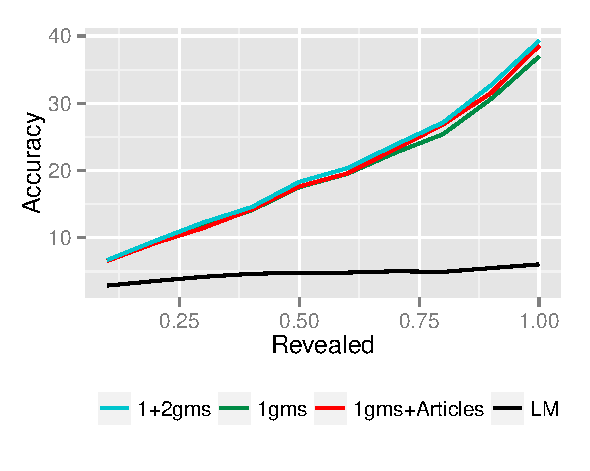
\includegraphics[width=1.0\linewidth]{2016_conll_verbpred/figures/german_top50_comparison}
\caption{German average prediction accuracy over the course of
  sentences. Bigrams help slightly in the second half of the sentence.
  Adding special features for case-assigning articles to unigrams
  nearly matches the performance of adding all bigrams in the final
  10\%. All handily outperform the trigram language
  model.}  \label{fig:german_unibi} \end{center}
\end{figure}

\paragraph{Richer Features Help (Mostly at the End)}

Bigram features help both languages, but Japanese more than German;
beyond bigrams, however, trigrams and longer features overfit the
training data and hurt performance.  The better performance for
Japanese bigrams is likely because word boundaries are not
well-defined in Japanese, and individual morphemes can combine in ways
that significantly add information.  German word boundaries are more
precise and words (particularly nouns) can carry substantial
information themselves.

Richer features matter more toward the end of the sentence.  In
Japanese, adding bigrams consistently outperforms unigrams alone, but
in both languages, adding special features for tokens with case
information helps almost as much as adding the full set of bigrams.
In Japanese, case markings always immediately follow the words marked,
and in German the articles precede the nouns to which they assign
case; thus, rather than relying on isolated unigrams, using bigrams
provides opportunities to encode case-marked words that more narrowly
select for verbs.  In Japanese, the differences are more pronounced
toward the very end of the sentences (and less so in German).


Richer features help more at the end, but not merely because the last
words of the sentence represent the densest feature vectors.  In
Japanese, the last word is usually a case-marked noun phrase or adverb
that matches the main predicate.  The final word is therefore immune
to subclause interference and must modify the final verb, boosting the
classifier performance in these final positions and amplifying the
predictive discrepancies between the various feature sets.  Accuracy
spikes at the end of Japanese sentences, where case information helps
nearly as much as adding the entire set of bigrams, further supporting
case information's importance.  Deeper processing---e.g., separating
case-marked words in subclauses from those in the main clause---would
likely be more useful.  Features and feature-selection strategies that
we tried which did not help included the following: adding only case
marker unigrams (instead of bigrams); filtering the features by using
only case-marked words; only allowing one word per case marker in the
feature vector (the most recent); using decaying weights on features
further in the past; adding part-of-speech tag $n$-grams; and adding
the word nearest to the centroid of the observed context in a word
embedding space.  While these features may have potential, they did
not lead to meaningful increases in accuracy in our experiments.

\begin{figure}[t!]
 \begin{center} 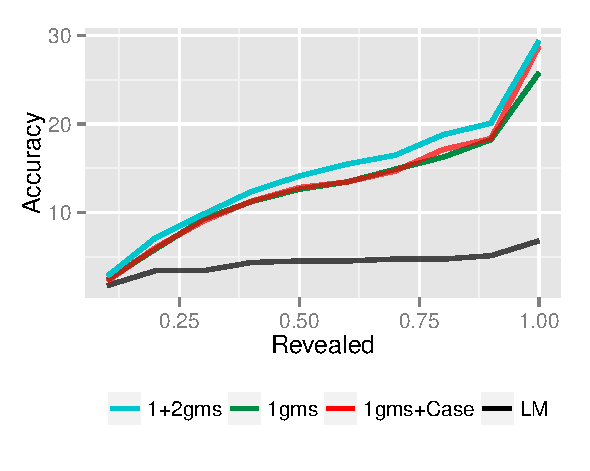
\includegraphics[width=1.0\linewidth]{2016_conll_verbpred/figures/japanese_top50_comparison_newsplit}
\caption{Japanese average prediction accuracy over the course of
  sentences. Adding bigrams consistently outperforms unigrams alone in
  Japanese, possibly due to the agglutinative nature of the language.
  The accuracies diverge the most toward the end of the sentences:
  Adding only explicit case markers to unigrams nearly matches
  performance of adding all bigrams toward the end. All outperform the
  trigram language model.}  \label{fig:japanese_unibi}
\end{center}
\end{figure}